\subsection{End-to-End Reinforcement Learning of Dialogue Agents for Information Access \cite{Dhingra2016End}}
The task is to provide a user with an sorted list of entities, which are believed to match the user goal, from a database through dialogue. The paper presents an end-to-end trainable system: \emph{KB-InfoBot}. The high-level overview of KB-InfoBot is shown in Figure \ref{fig:Dhingra2016End01}.

\begin{figure}[htbp]
  \centering
  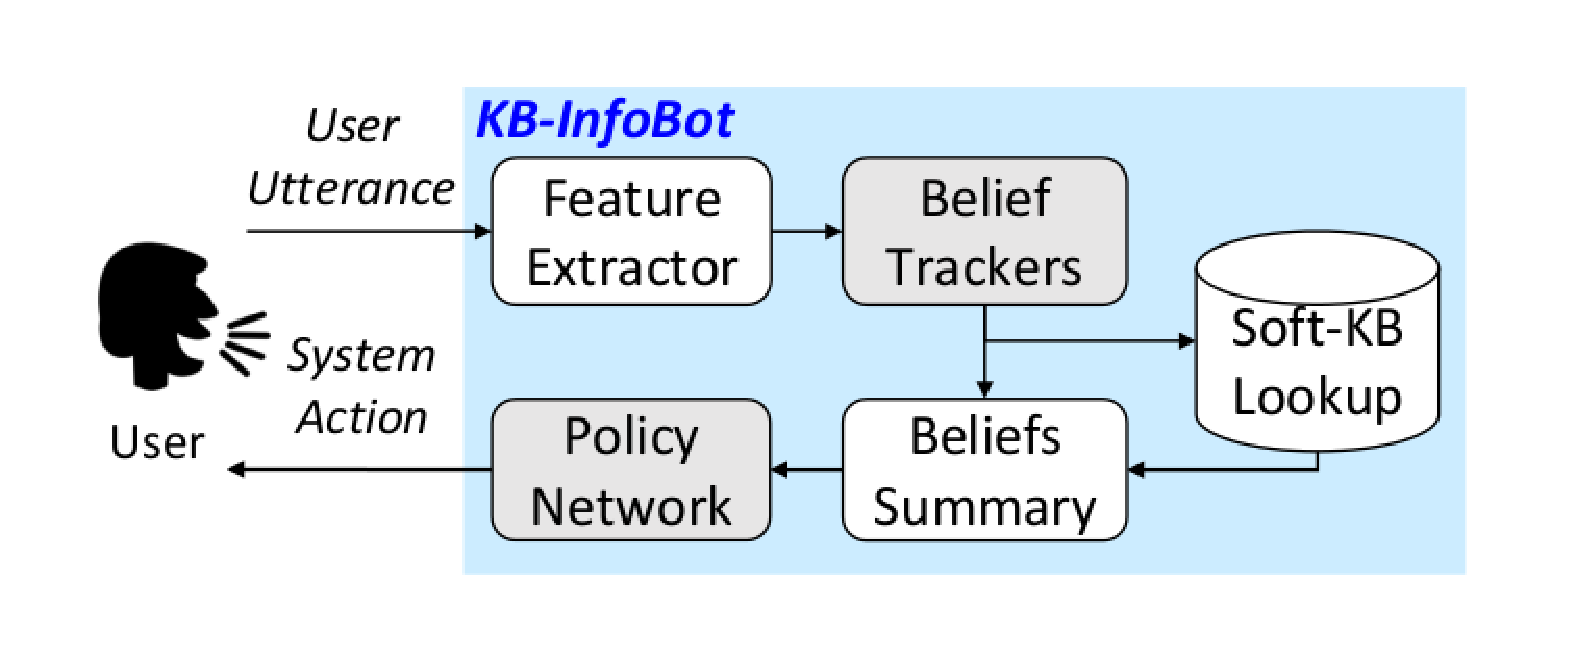
\includegraphics[width=0.8\linewidth]{Dhingra2016End01}
  \caption{KB-InfoBot}
	\label{fig:Dhingra2016End01}
\end{figure}

Assuming that in the database, there are $N$ entities, each of which has $M$ slots. At each turn, the input is an user utterance $u^{t}$ and the output is a system action $a^{t}$. The action space $\mathcal{A}$ has $M+1$ actions: (1) \emph{request($s_{j}$)} asking the user for the value of slot $j$ for $1 \leq j \leq M$; (2) \emph{inform($I$)} showing an sorted list of entities to the user. Each component of KB-InfoBot is defined as follows:

\begin{itemize}
\item[-] \textbf{Feature Extractor} converts $u^{t}$ into a vector representation $x^{t}$, each element of which indicates the count of a certain 2-gram in $u^{t}$. The vocabulary size is 3078 and thus $x^{t}$ is a 3078-dimensional vector.

\item[-] \textbf{Belief Tracker} takes $x^{t}$ as input and for each slot, updates the internal representation $h^{t}_{j}$ and outputs the belief state $p^{t}_{j}$ and $q^{t}_{j}$. The internal representation starting from $h^{0}_{j}=\mathbf{0}$ is updated by a Gated Recurrent Unit:
\begin{equation}
\begin{aligned}
r^{t}_{j} \ =& \ \sigma( W^{r}_{j}x^{t} + U^{r}_{j}h^{t-1}_{j} + b^{r} ) \\
z^{t}_{j} \ =& \ \sigma( W^{z}_{j}x^{t} + U^{z}_{j}h^{t-1}_{j} + b^{z} ) \\
h^{t}_{j} \ =& \ (1-z^{t}_{j}) \odot h^{t-1}_{j} + z^{t}_{j} \odot \tanh( W^{h}_{j}x^{t} + U^{h}_{j}(r^{t}_{j} \odot h^{t-1}_{j}) + b^{h} ) \\
\end{aligned}
\end{equation}
Then, the belief state is computed:
\begin{equation}
\begin{aligned}
p^{t}_{j} \ =& \ softmax( W^{p}_{j}h^{t}_{j} + b^{p}_{j} ) \\
q^{t}_{j} \ =& \ \sigma( W^{q}_{j}h^{t}_{j} + b^{q}_{j} ) \\
\end{aligned}
\end{equation}
where $p^{t}_{j}$ is a multinomial distribution over all the possible values of slot $j$, and $q^{t}_{j}$ is a bernoulli distribution indicating whether the user know the value of slot $j$ or not.

\item[-] \textbf{Soft-KB Lookup} uses $p^{t}_{j}$ and $q^{t}_{j}$ to compute $p^{t}$, the posterior distribution over the entities in the database:
\begin{equation}
p^{t}(i) \ \propto \ \prod_{j=1}^{M} p^{t}_{j} (i) \\
\end{equation}
which is the posterior probability that the $i$th entity is targeted by the user.
\[
    p^{t}_{j}(i) \ = \
\begin{cases}
    \frac{1}{N},                                                                                     & \text{if } i \in M_{j} \\
    q^{t}_{j}\frac{p^{t}_{j}(i_{j})}{N_{j}(i_{j})} (1- \frac{|M_{j}|}{N}) + (1-q^{t}_{j})\frac{1}{N},& \text{otherwise}
\end{cases}
\]
where $N_{j}(i_{j})$ is the count of value $i_{j}$ in slot $j$, and $M_{j}$ is the set of entities for which the value of slot $j$ is missing.

\item[-] \textbf{Beliefs Summary} summarizes slot $j$ into an entropy statistic, $H(p^{t}_{j})$, over a distribution $w^{t}_{j}$:
\begin{equation}
w^{t}_{j}(v) \ \propto \ \sum_{i:i_{j}=v} p^{t}(i) + p^{0}_{j}(v) \sum_{i:i_{j}\ is\ missing} p^{t}(i) \\
\end{equation}
In a similar way, $p^{t}$ is summarized into $H(p^{t})$. The summary vector $s^{t}=[H(p^{t}_{1}), ..., H(p^{t}_{M}), q^{t}_{1}, ..., q^{t}_{M}, H(p^{t})]$ is input to the policy network.

\item[-] \textbf{Policy Network} selects the next action based on the dialogue history and the current summary vector $s^{t}$:
\begin{equation}
\begin{aligned}
h^{t}_{\pi} \ =& \ GRU( s^{1}, ..., s^{t} ) \\
\pi \ =& \ softmax( W^{\pi}h^{t}_{\pi} + b^{\pi} ) \\
\end{aligned}
\end{equation}

\item[-] \textbf{Action Selection} samples the next action from the polity $\pi$. If action \emph{inform()} is chosen, an ordered list $I=(i_{1}, ..., i_{R})$ of indices is provided to the user.
\end{itemize}